\subsection{The Second Refinement}
\label{sec:component_diagrams-tutorial_secondRefinement}


The washing machine sub-system component is now further refined, as shown in Figure \ref{fig:SecondRefinementOfWashingMachine}, into two components, the DOOR sub-system and an abstract component, WM, that represents the rest of the washing machine sub-system. Two connectors enable communication between these two components. The first, lock, passes a Boolean signal to the DOOR sub-system to lock the door. The second, doorPosition, informs the Washing Machine sub-system when the door is opened or closed.
 
 \begin{figure}[!htbp]
  \centering
  \ifplastex
  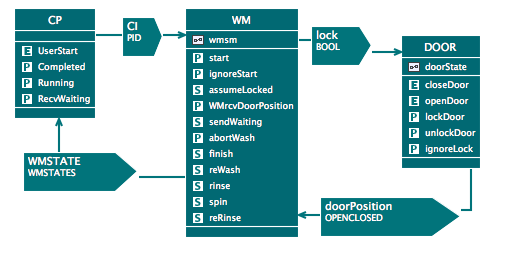
\includegraphics[width=1024]{figures/image25.png}
  \else
  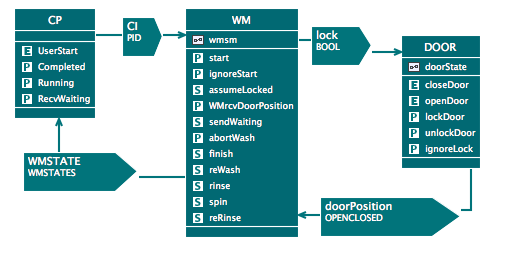
\includegraphics[width=1\textwidth]{figures/image25.png}
  \fi
  \caption{Second Refinement of Washing Machine}
  \label{fig:SecondRefinementOfWashingMachine}
\end{figure} 

Note that the  \code{DOOR} component has two external operations, closeDoor and openDoor, which represent the interaction of the user with the door. Care is needed in this refinement to ensure that the system cannot get into an unsafe state; the door should always be locked when the washing machine is washing, rinsing or spinning so that the user cannot inadvertently open the door and release potentially very hot water.
The state-machine for the washing machine is refined to split the  \code{WASHING} state into sub-states  \code{LOCKINGDOOR} and  \code{INPROGRESS} and  \code{IDLE} into  \code{UNLOCKINGDOOR} and  \code{IDLEWAITING}, Figure \ref{fig:SecondRefinementRefinedStatemachineOfTheWashingMachine}. This is necessary to accommodate the new transitions concerned with locking and unlocking the door.
 
 \begin{figure}[!htbp]
  \centering
  \ifplastex
  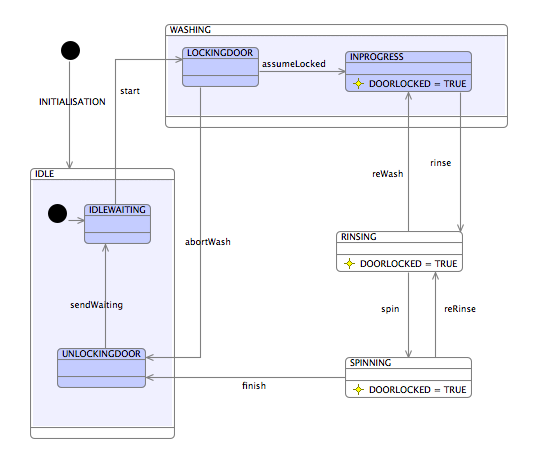
\includegraphics[width=1024]{figures/image26.png}
  \else
  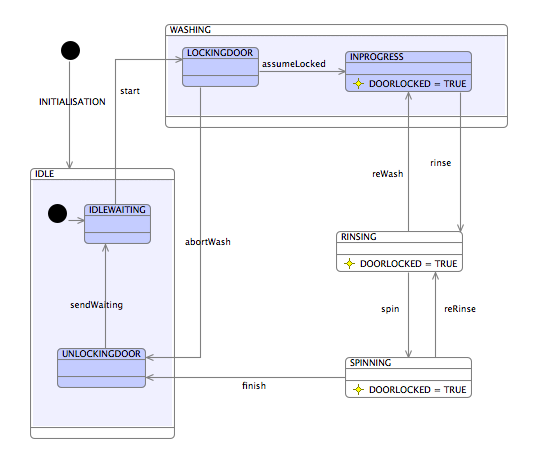
\includegraphics[width=1\textwidth]{figures/image26.png}
  \fi
  \caption{Second Refinement : Refined State-machine of the Washing Machine}
  \label{fig:SecondRefinementRefinedStatemachineOfTheWashingMachine}
\end{figure} 

An invariant,  \code{DOORLOCKED  = TRUE}, is introduced in the sub-system state machine for states  \code{INPROGRESS},  \code{RINSING} and  \code{SPINNING}.
The state machine for the door sub-system is shown in Figure \ref{fig:SecondRefinementStatemachineForTheDoorComponent}. The door may be open ( \code{DOOROPEN}) in which case any instructions to lock the door are ignored ( \code{ignoreLock}) or it may be closed ( \code{DOORCLOSED}). When the door is closed it may be unlocked ( \code{DOORUNLOCKED}) or locked ( \code{DOORLOCKED}). Note that the transitions  \code{unlockDoor} and  \code{lockDoor} are drawn with the superstate  \code{DOORCLOSED} as their source indicating that they can fire irrespective of whether the door is locked or not.
 
 \begin{figure}[!htbp]
 \centering
      \ifplastex
      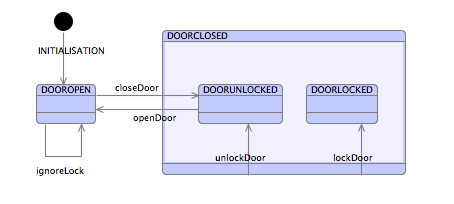
\includegraphics[width=1024]{figures/image27.png}
      \else
      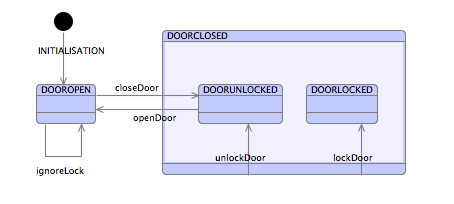
\includegraphics[width=1\textwidth]{figures/image27.png}
      \fi
  \caption{Second Refinement : State-machine for the Door Component}
  \label{fig:SecondRefinementStatemachineForTheDoorComponent}
\end{figure} 

The washing machine sub-system sends a message via the lock connector to the door sub-system to lock the door if it has received a message from the door via the doorPosition connector indicating that the door is closed.  The washing machine sub-system then initiates a self-wake, delayed by 3 time units, as shown in Figure \ref{fig:SecondRefinementSelfWakeToCheckDoorLocked}. If the door is still closed at the self-wake, as indicated by the guard 
 \code{WM\_doorPosition = CLOSED},  then it is assumed that the door is locked and the system can proceed to the  \code{INPROGRESS} state. The alternative transition (Figure \ref{fig:SecondRefinementRefinedStatemachineOfTheWashingMachine}) is abortWash which has the negated guard  \code{WM\_doorPosition $\neq$ CLOSED}.
 
 \begin{figure}[!htbp]
  \centering
  
   \subfloat[initiate self-wake]{
      \ifplastex
      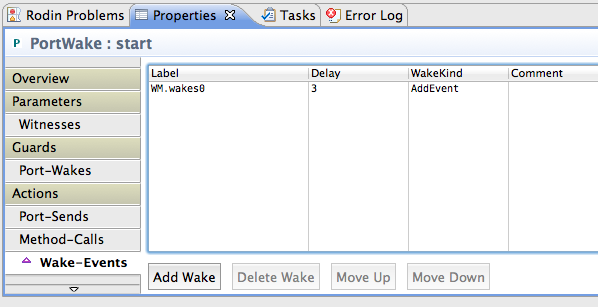
\includegraphics[width=1024]{figures/image28.png}
      \else
      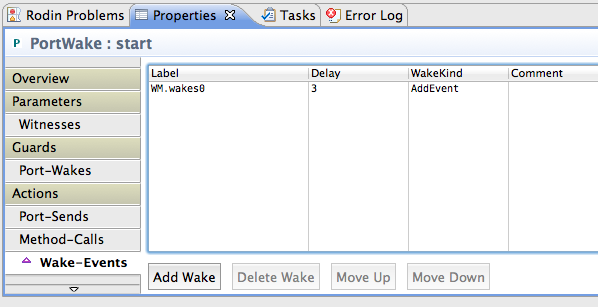
\includegraphics[width=1\textwidth]{figures/image28.png}
      \fi
  }
      
  \subfloat[respond to self-wake]{
     \ifplastex
     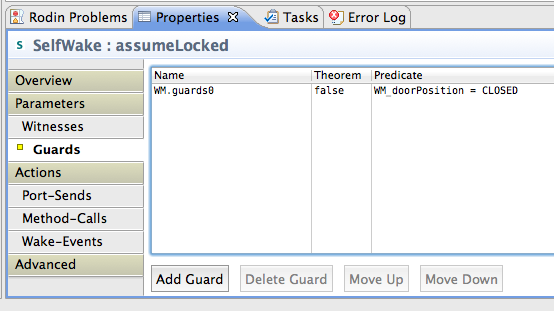
\includegraphics[width=1024]{figures/image29.png}
     \else
     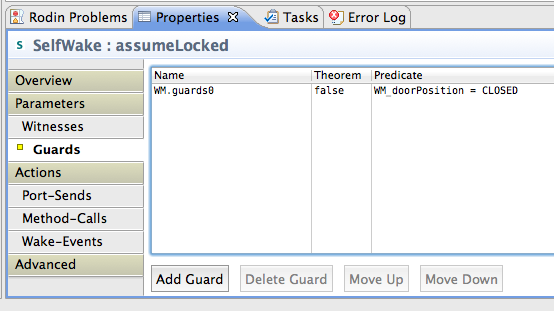
\includegraphics[width=1\textwidth]{figures/image29.png}
     \fi
  }
  
  \caption{Second Refinement : Self Wake to Check Door Locked}
  \label{fig:SecondRefinementSelfWakeToCheckDoorLocked}
\end{figure} 

The proof obligations generated for the safety invariant are difficult to discharge. It is a good idea at this stage to proceed immediately to animation and model checking, to ensure that the model behaves as expected.
Model checking does indeed show immediately that the safety invariant is violated and provides a counterexample in the history pane as shown in Figure \ref{fig:CounterexampleDiscoveredByProB}.
 
 \begin{figure}[!htbp]
  \centering
  \ifplastex
  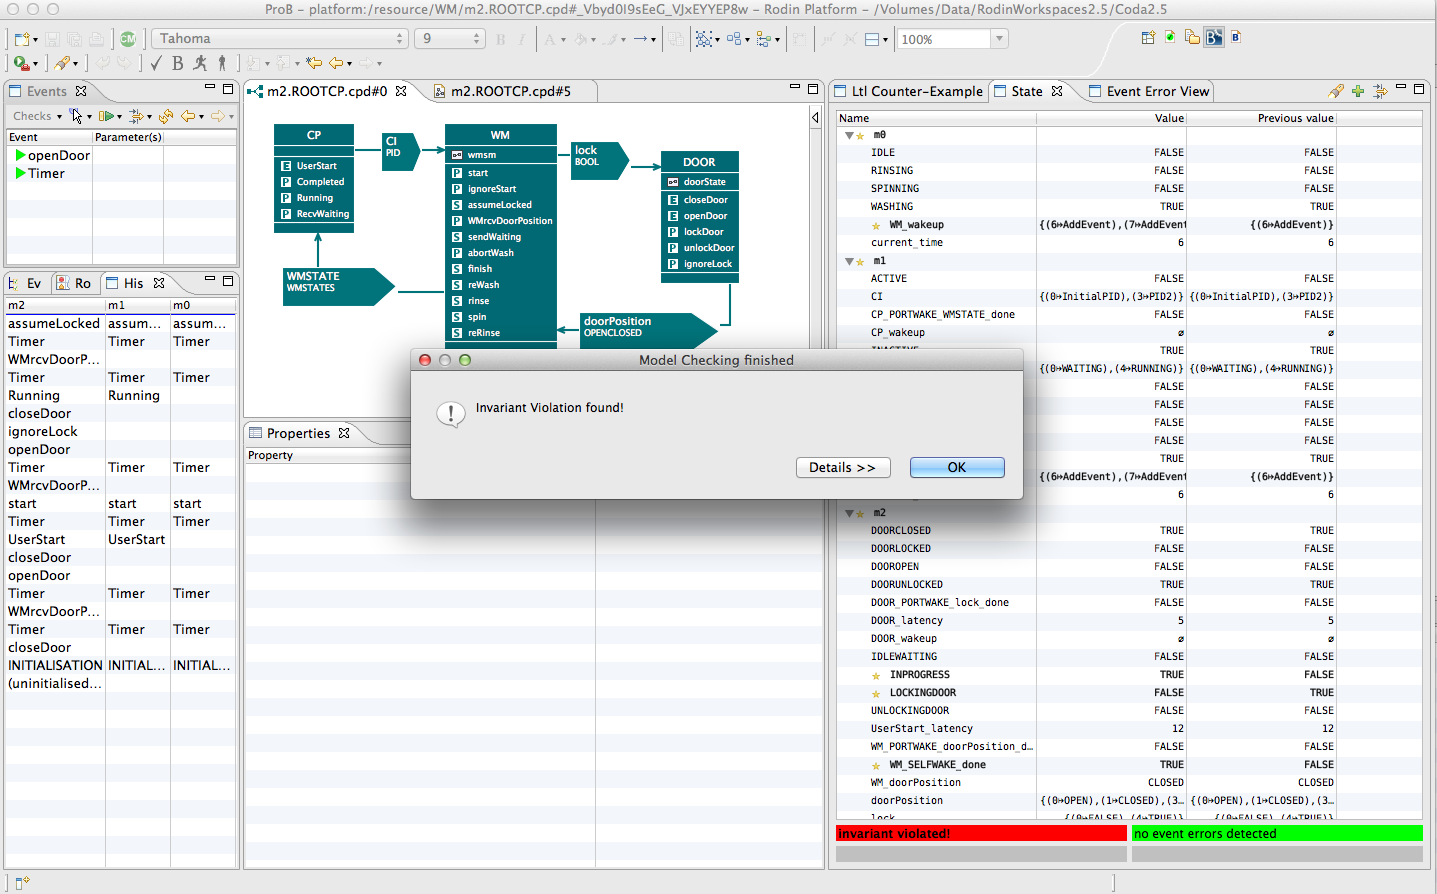
\includegraphics[width=1024]{figures/image31.png}
  \else
  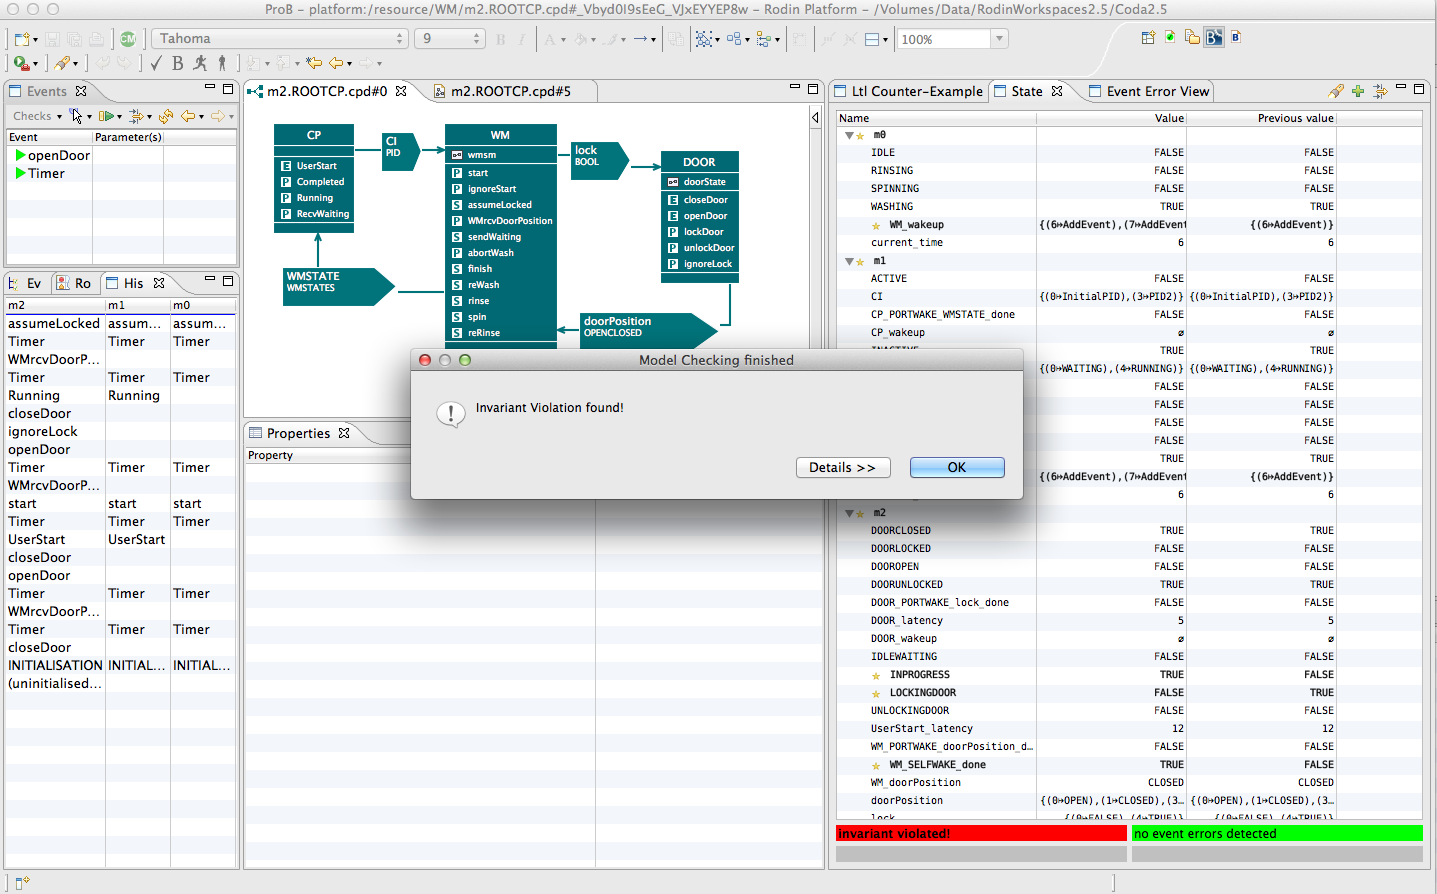
\includegraphics[width=1\textwidth]{figures/image31.png}
  \fi
  \caption{Counterexample Discovered by ProB}
  \label{fig:CounterexampleDiscoveredByProB}
\end{figure} 

Although the refinement models the latency that certainly exists between the washing machine sub-system and door sub-system, it allows the user to open and close the door repeatedly in zero-time. Modelling this Zeno Behaviour is unrealistic and results in a scenario where the user can close the door and then open it again immediately just before it is locked.
The solution is to model more realistically the latency that must exist in the opening and closing of the door by introducing a delay on the External Event, closeDoor, as shown in Figure \ref{fig:IntroducingLatencyToTheDoorOperations}. The guard  \textbf{\code{current\_time > DOOR\_latency}}, where \code{DOOR\_latency} is a variable that is set to \code{current\_time + 1} by any preceding door open or close events, ensures that two door events cannot occur on consecutive clock ticks. This corresponds to an assumption that the systems time response makes it impossible to open and close the door without it being detected. This is sufficient to ensure that any changes of door state are successfully transmitted to the WM component.
 
 \begin{figure}[!htbp]
  \centering
  \ifplastex
  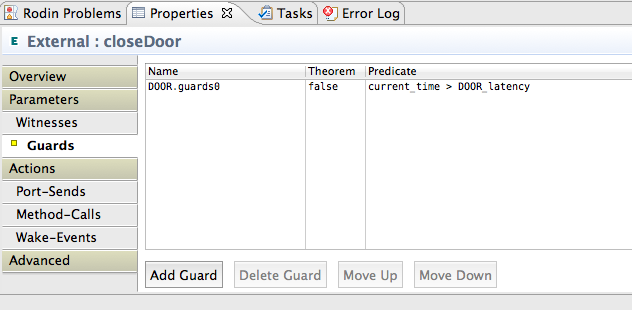
\includegraphics[width=1024]{figures/image32.png}
  \else
  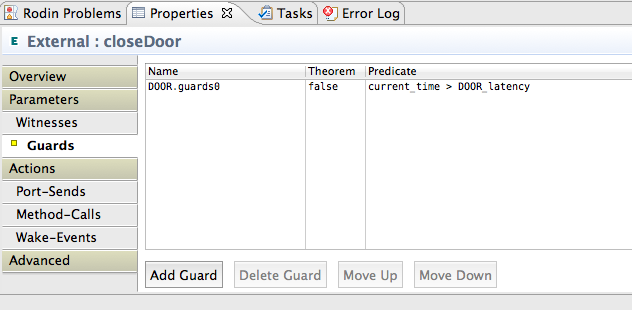
\includegraphics[width=1\textwidth]{figures/image32.png}
  \fi
  \caption{Introducing Latency to the Door Operations}
  \label{fig:IntroducingLatencyToTheDoorOperations}
\end{figure} 
 
The model checker is re-run to verify that the invariant violation has been addressed and that there is no deadlock, as shown in Figure \ref{fig:ProBModelCheckingCoverageForTheSecondRefinement}. Note now, that the model checking results show that not all operations have been covered, though examination of the guards and actions of these uncovered operations show that none are material to the invariant violation being investigated. Although not a proof, model checking with operation coverage gives confidence that the model is behaving as expected.
 
 \begin{figure}[!htbp]
  \centering
  \ifplastex
  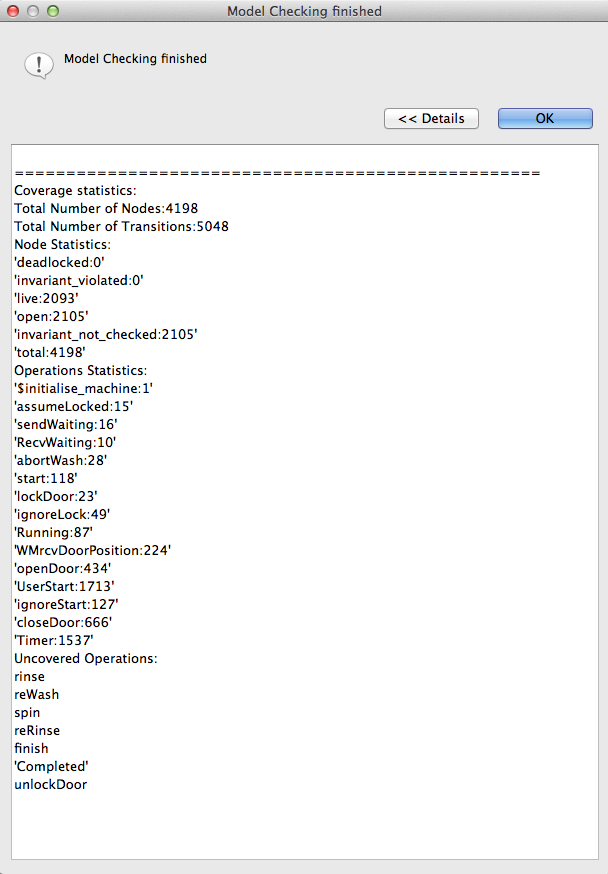
\includegraphics[width=1024]{figures/image33.png}
  \else
  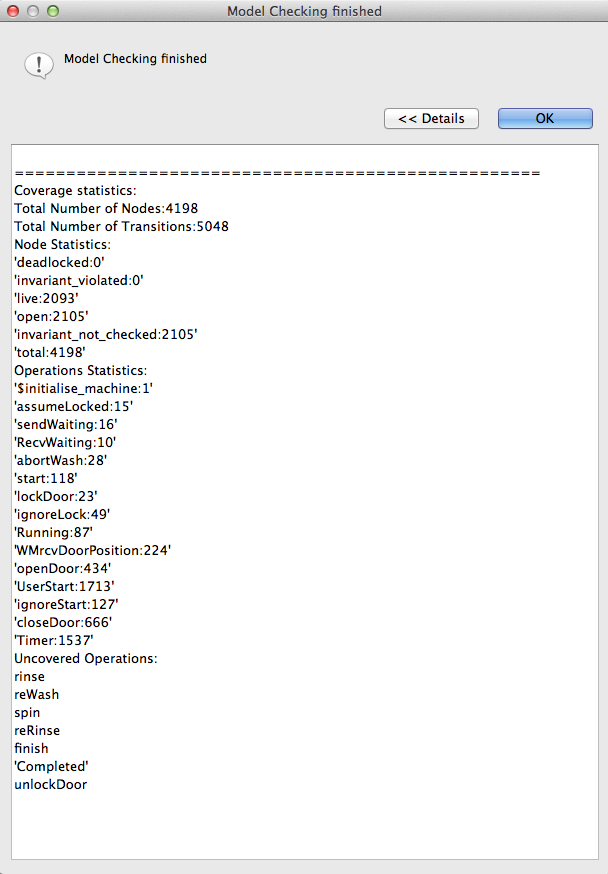
\includegraphics[width=1\textwidth]{figures/image33.png}
  \fi
  \caption{ProB Model Checking Coverage for the Second Refinement }
  \label{fig:ProBModelCheckingCoverageForTheSecondRefinement}
\end{figure} 
 
To improve operation coverage, it is a good idea to try the alternative Breadth First Search option. Figure \ref{fig:ProBModelCheckingCoverageForTheSecondRefinementBreadthFirst} shows the improved coverage results and Figure \ref{fig:ConfigurationForProBModelCheckerBreadthFirstOption} shows how this option is set.
 
 \begin{figure}[!htbp]
  \centering
  \ifplastex
  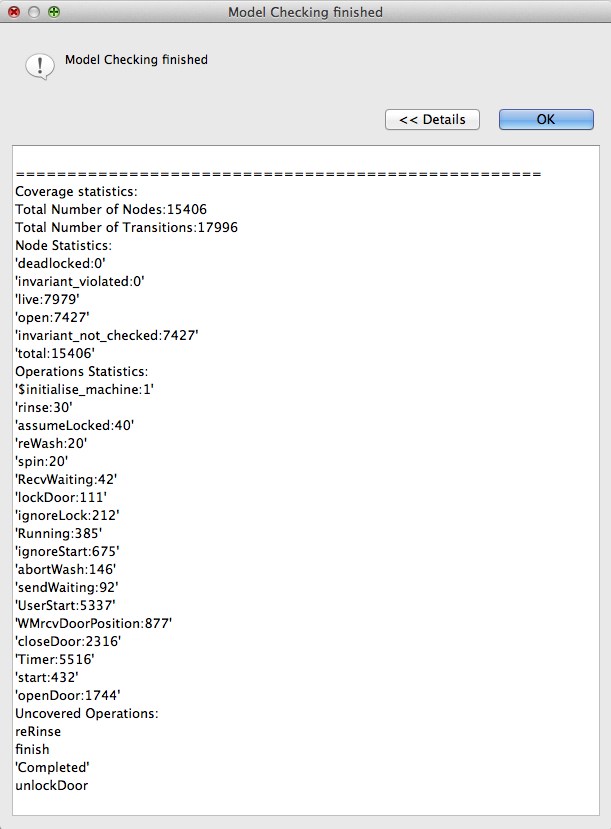
\includegraphics[width=1024]{figures/image34.png}
  \else
  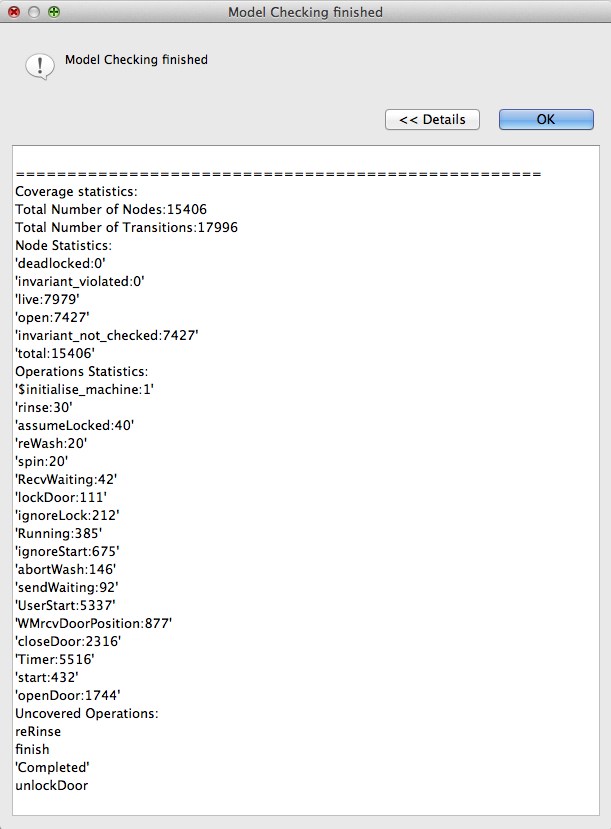
\includegraphics[width=1\textwidth]{figures/image34.png}
  \fi
  \caption{ProB Model Checking Coverage for the Second Refinement : Breadth First}
  \label{fig:ProBModelCheckingCoverageForTheSecondRefinementBreadthFirst}
\end{figure} 
 
 \begin{figure}[!htbp]
  \centering
  \ifplastex
  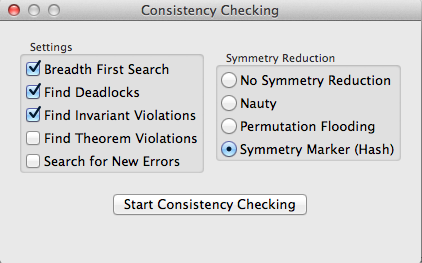
\includegraphics[width=1024]{figures/image35.png}
  \else
  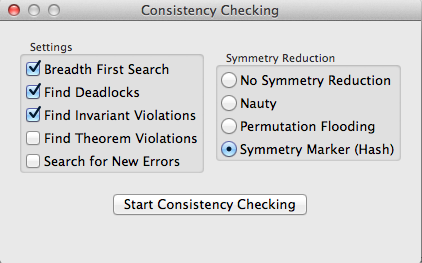
\includegraphics[width=1\textwidth]{figures/image35.png}
  \fi
  \caption{Configuration for ProB Model Checker Breadth First Option}
  \label{fig:ConfigurationForProBModelCheckerBreadthFirstOption}
\end{figure} 
 
%%% Local Variables:
%%% mode: latex
%%% TeX-master: "component_diagrams-user_manual"
%%% End:
